
% TODO
% Fix ref to : - CodeOcean. (2018). "What is a compute capsule?" Downloaded from https://help.codeocean.com/getting-started/what-is-a-compute-capsule

\documentclass[conference]{IEEEtran}

\IEEEoverridecommandlockouts
% The preceding line is only needed to identify funding in the first footnote. If that is unneeded, please comment it out.

\usepackage{cite}
\usepackage{amsmath,amssymb,amsfonts}
\usepackage{algorithmic}
\usepackage{graphicx}
\usepackage{textcomp}
\usepackage{xcolor}
\usepackage[utf8]{inputenc}
\usepackage[T1]{fontenc}

\def\BibTeX{{\rm B\kern-.05em{\sc i\kern-.025em b}\kern-.08em
  T\kern-.1667em\lower.7ex\hbox{E}\kern-.125emX}}

\begin{document}

\title{
  Preserving Reproducibility: Provenance and Executable Containers in DataONE Data Packages
  \thanks{Funding support for the work described in this paper was provided by National Science Foundation awards 1430508, 1541450, and 1262458. Additional support was provided by the National Center for Ecological Analysis and Synthesis, a Center funded by the University of California, Santa Barbara, and the State of California.}
}

\author{
  \IEEEauthorblockN{Bryce Mecum}
  \IEEEauthorblockA{
  	\textit{National Center for Ecological}\\\textit{Analysis and Synthesis}\\
  	\textit{Univ. of California, Santa Barbara}\\
  	Santa Barbara, California, United States \\
  	mecum@nceas.ucsb.edu\\
  	https://orcid.org/0000-0002-0381-3766
  }
\and
  \IEEEauthorblockN{Matthew B. Jones}
  \IEEEauthorblockA{
  	\textit{National Center for Ecological}\\
    \textit{Analysis and Synthesis}\\
  	\textit{Univ. of California, Santa Barbara}\\
  	Santa Barbara, California, United States \\
  	jones@nceas.ucsb.edu\\
  	https://orcid.org/0000-0003-0077-4738
  }
\and
  \IEEEauthorblockN{Dave Vieglais}
  \IEEEauthorblockA{
  	\textit{Biodiversity Institute \&}\\
  	\textit{Natural History Museum}\\
  	\textit{University of Kansas}\\
  	Lawrence, Kansas, United States\\
  	vieglais@ku.edu\\
  	https://orcid.org/0000-0002-6513-4996
  }
\and
  \IEEEauthorblockN{Craig Willis}
  \IEEEauthorblockA{
  	\textit{School of Information Sciences}\\
  	\textit{University of Illinois}\\
  	Champaign, Illinois, United States \\
  	willis8@illinois.edu\\
  	https://orcid.org/0000-0002-6148-7196
  }
}

\maketitle

\begin{abstract}
  Many data packaging standards are available to researchers and data repository operators and the choice to use an existing standard or create a new one is challenging. We introduce the DataONE Data Package standard which is based on the existing OAI-ORE Resource Map standard. We describe the functionality Data Package provides, implementation considerations, compare it to existing standards, and discuss future extensions to the standard including the ability to describe execution environments via WholeTale ``Tales``'' and alternate serialization formats.
\end{abstract}

\begin{IEEEkeywords}
  data packaging, standards, OAI-ORE, reproducibility, DataONE, WholeTale
\end{IEEEkeywords}

\section{Introduction}

Many formats and standards for packaging research objects exist, each with communities of practice, nomenclature, intended use cases, and target audiences.
All of these formats share the common goal of grouping together the digital artifacts of scientific research into a packaging format of some form or another.
DataONE\footnote{https://www.dataone.org/} refers to these composites as Data Packages\footnote{https://releases.dataone.org/online/api-documentation-v2.0/design/DataPackage.html} (and the individual artifacts as Data Objects) which contain artifacts such as data, metadata, software, and other products of research such as figures and model output (Fig. \ref{dataone-data-package}).

\begin{figure}[ht]
	\centerline{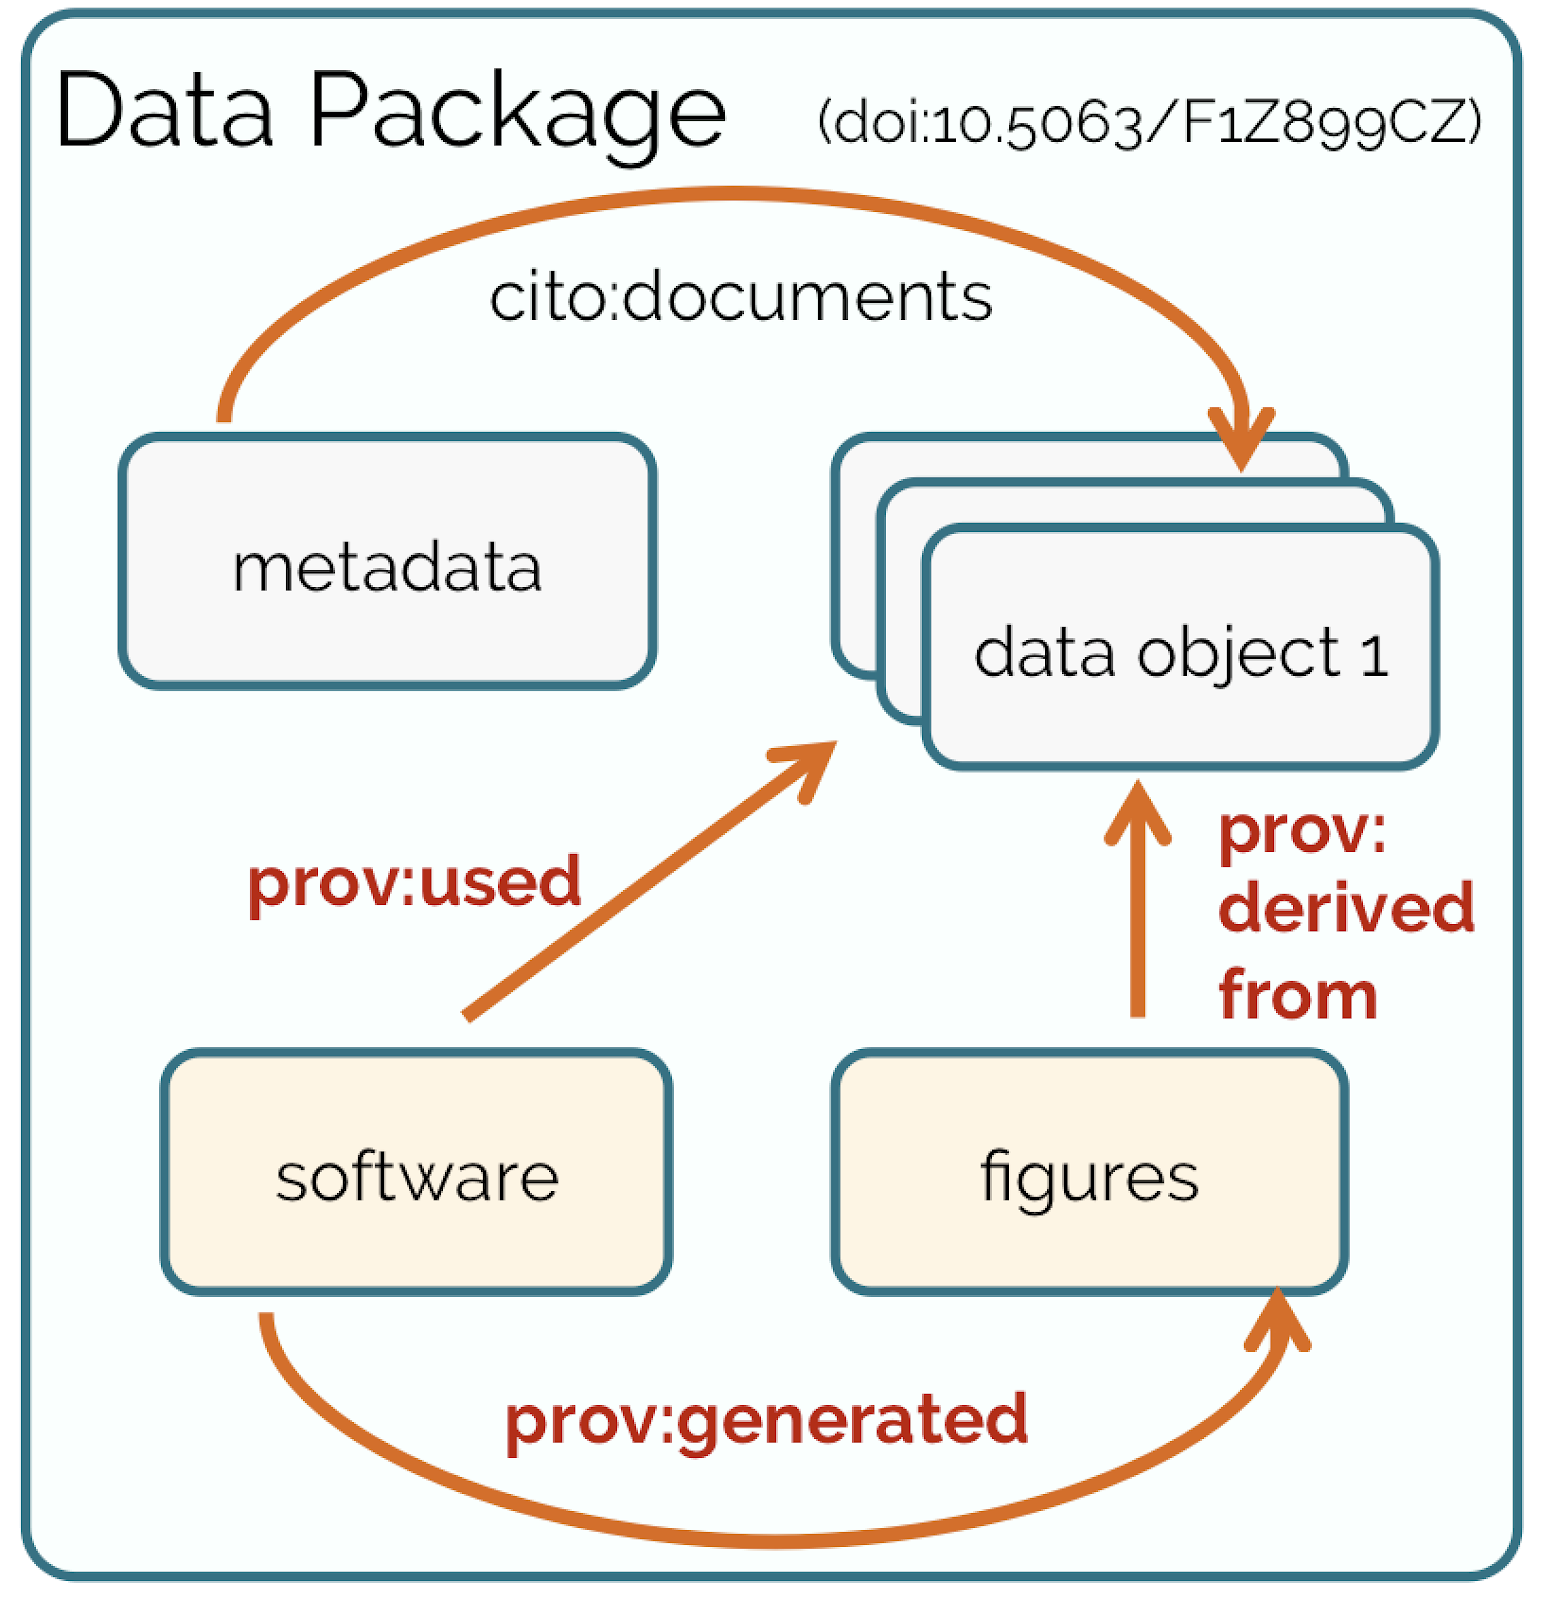
\includegraphics[width=0.5\textwidth]{dataone-data-package.png}}
	\caption{A DataONE Data Package is a composite container for data, software, and visualizations, and the metadata that describes these.  Provenance relationships link the objects within and across Data Packages into computational workflows for reproducible science.}
	\label{dataone-data-package}
\end{figure}

In addition to packaging together the artifacts of research, some packaging formats also provide additional features such as rich metadata using XML schemas, provenance, and multiple serialization formats.
With so many existing packaging formats, choosing a particular packaging format is a challenging task for both researchers and data repository operators alike.

DataONE is a federation of data repositories that federates data and metadata from over 45 data repository systems.
DataONE provides data packaging for composite research outputs via an extension of the well-established Open Archives Initiative Object Reuse and Exchange (OAI-ORE) \cite{lagoze2012} Resource Map standard (hereafter, Resource Map), and optionally supports serialization using BagIt\footnote{https://tools.ietf.org/html/draft-kunze-bagit-16}. 
From its inception, DataONE made use of established and open standards where practical in order to maximize interoperability.
Resource Maps provided an open and standardized format for describing aggregations of resources on the web by using their respective Uniform Resource Identifiers (URIs) to provide linkages in a Resource Description Framework (RDF) model. Resource Maps use RDF predicates to provide relationships between aggregated components, enabling tremendous flexibility for describing package constructs and any annotations therein (such as provenance). DataONE’s Data Package specification is a convention using Resource Maps with a set of additional constraints on top of the standard to improve preservation, access, and linking of Data Packages:

\begin{enumerate}
  \item{When serializing a Data Package in BagIt format, the Resource Map must be serialized in RDF/XML format with a particular filename in the BagIt bag.}
  \item{Each resource with a representation in a Data Package MUST be described with a \texttt{dcterms:identifier} containing the DataONE persistent identifier.}
  \item{All DataONE Objects in the Resource Map MUST be expressed as a URI using DataONE’s resolving service, instead of using a URI to a specific replica on a repository. This is to separate the current physical location of a resource from its identity.}
  \item{A mapping between the \texttt{dcterms:identifier} and the file location in the BagIt \texttt{data} directory must be provided in a manifest file named \texttt{pid-mapping.txt}. This allows a direct correspondence to be discovered between local objects in a serialized bag and remote resource URIs in the Resource Map document by using the persistent identifier to link them.}
  \item{The aggregation resource URI SHOULD be expressed as a hash URI based on the Resource Map URI, as recommended by ORE\footnote{http://www.openarchives.org/ore/1.0/primer\#remHashURIs}\footnote{http://www.openarchives.org/ore/1.0/http\#Simple}. This ensures that the aggregation can be referenced directly in other Resource Maps and still be resolved.}
  \item{When referencing another DataONE Data Package, the URI of the Data Package being referenced MUST resolve to a Resource Map. The URI can either be the Resource Map URI or the aggregation URI if it follows the hash URI format. Since some existing Resource Maps do not use aggregation URI’s that resolve to the Resource Map, it is necessary to check their format before deciding which to use.}
  \item{When expressing an identifier in a URI, it must be URL encoded. When expressing in the \texttt{dcterms:identifier} field, it must not (although appropriate XML encoding applies).}
  \item{The Resource Map MUST assert a statement with the \texttt{ore:isDescribedBy} relationship between the Resource Map and the aggregation, following the recommendation that aggregations with multiple resource maps express this relationship\footnote{http://www.openarchives.org/ore/1.0/datamodel\#ReM-to-aggr}.}
\end{enumerate}

These rules, while minor, allow DataONE to successfully federate a collection of research objects and their associated metadata as a DataONE Data Package and provide effective search and discovery tools for researchers.
The decision to re-use an existing standard has multiple advantages: (1) Data Packages can be parsed and serialized by existing, well-tested software tools, and (2) Data Packages have meaning outside of DataONE’s Data Package standard in that they can be treated as Resource Maps and are therefore interoperable with similar systems supporting Resource Maps without the need to specifically support DataONE Data Packages.

\section{Incorporating Provenance in Packages}

Archiving the input and output objects of research for later access is a key piece of a reproducible scientific process.
However, without information about how those research objects came into existence and relate to one another, the research is likely not reproducible by another scientist.
For example, one needs to know which computational processes used which input objects, which software was used to execute the computation, and which output objects were produced, often in a complex workflow consisting of hundreds of steps.

To address this problem, DataONE includes provenance information in datasets as part of the enclosing Data Package.
In doing this, DataONE created ProvONE\footnote{https://purl.dataone.org/provone-v1-dev}, a Web Ontology Language (OWL) ontology that extends the W3C PROV\footnote{https://www.w3.org/TR/prov-overview/} standard for describing the provenance of computational workflows.
ProvONE represents provenance information in the form of RDF/XML that is inserted in the Resource Maps that define Data Packages.
Adding provenance to a Data Package in this way is straightforward because Resource Maps are already modeled with RDF and therefore can include other arbitrary models such as ProvONE.

\begin{figure}[ht]
\centerline{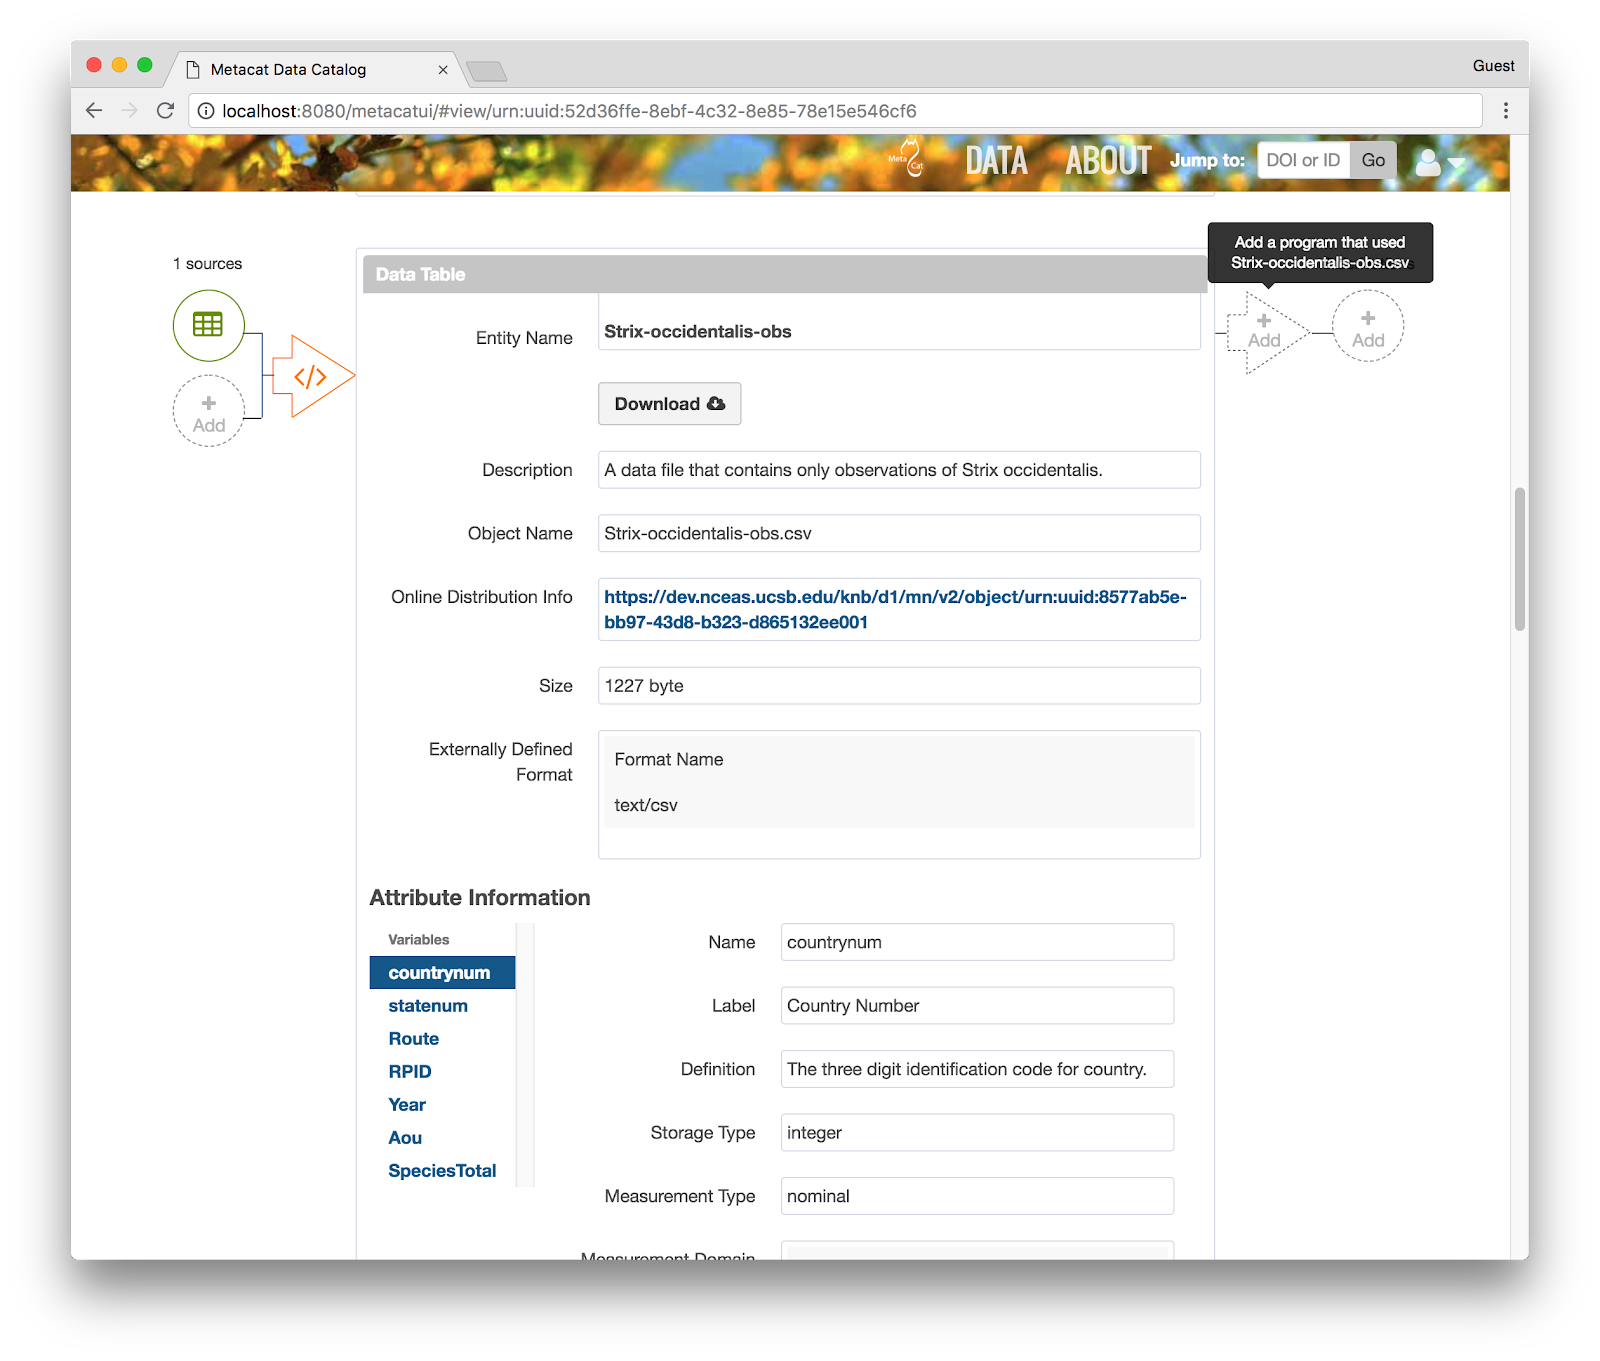
\includegraphics[width=0.5\textwidth]{prov-editor.png}}
\caption{DataONE provides rich web displays and editing of provenance information contained in its Data Packages.}
\label{prov-editor}
\end{figure}

To assist scientists in creating and consuming this provenance information, DataONE provides a rich web display (Fig.~\ref{prov-editor}) on Data Package landing pages and two packages for the R Programming Language \cite{rcoreteam2018}: \texttt{recordr}\footnote{https://github.com/NCEAS/recordr} for automatically recording provenance during R sessions, and \texttt{datapack}\footnote{https://github.com/ropensci/datapack}, for serializing provenance information into Data Packages.
Together, the Data Package model and ProvONE model, along with accompanying support in user-facing software tools, enable researchers to effectively describe the content and provenance of their research outputs.

\section{Implementation considerations}

While making use of the existing Resource Map standard for packaging in DataONE has had advantages, the choice was not without the need for careful implementation.
Designing a new packaging standard might have been easier due to not having to consider interoperability with other communities and being able to optimize the standard against technology stacks for performance reasons.
However, Resource Maps have been well-suited to the needs of the Data Package standard with only minor implementation considerations needed along the way.

The first consideration was building effective search and discovery interfaces based upon Resource Maps.
Because Resource Maps support the full semantic and logical richness of RDF and OWL, it was tempting to make the search indexes behind DataONE’s search interfaces support that same level of richness.
Existing tools for processing Resource Maps\footnote{https://github.com/abrin/foresite-toolkit} work well for smaller packages but exhibit exponential increases in processing time and computing resource usage for larger (> 1000 object) packages.
To work around these performance issues, some member repositories in DataONE artificially limited the number of objects that can be included in Data Packages, even though science is often done at a scale beyond 1000 objects.

The second implementation consideration is dealing with the inherently flat nature of Resource Maps: All resources in the Resource Map are described at the same level of hierarchy (i.e., in an Aggregation).
However, scientists often arrange their research in a hierarchy of files and folders that confers important semantic relationships among the artifacts and their use in the research.
Numerous repositories approach this limitation by making use of nested Resource Maps to match the nested structure of filesystems, where each level of hierarchy is described by a separate Resource Map that can contain other Resource Maps representing child folders.
This has worked, but was difficult to implement across DataONE's software tooling for two reasons:
First, because all DataONE objects are immutable and have their own unique identifiers, adding or changing the identifier of a child Resource Map requires an update all parent Resource Maps up to the topmost parent in the Data Package hierarchy, which is computationally intensive and requires careful implementation in software tools.
Second, because the Data Package specification requires each Data Package to have at least one metadata record aggregated within it, metadata records throughout complex hierarchies tended to either be too minimal to support standalone interpretation and/or contained highly-redundant information which made it hard for users to discern between Data Packages in search interfaces.

The third implementation consideration is less specific to Resource Maps and more due to the interaction between Resource Maps and the DataONE Objects (which Data Packages aggregate).
In DataONE, any changes in the content of an Object requires a new identifier for the Object, and, thus, building user-facing tools that do both the right thing and won’t surprise users requires careful consideration.
For example, if a user authors a Data Package with a metadata record describing an Excel spreadsheet and they decide to replace the Excel spreadsheet with a Comma-Separated Values (CSV) version of the same data, do existing references to the Excel file in the Resource Map (which were asserted by URI) still apply to the CSV version of the package?
Should the RDF triples that referenced the Excel spreadsheet be automatically removed for the user?
Or if the user has provenance information embedded in their Resource Map and they author provenance that details an R script that generated a figure, what happens in the Resource Map if they update the R script (resulting in a new DataONE Object with a new identifier)?
Should the statement connecting the previous version of the R script be removed or updated to connect the new version?
Should both be retained?
These kinds of problems are tractable, but need careful attention in user interfaces to make it clear to the user what changes their actions are going to cause and to provide sensible defaults.

\section{Comparison with other packaging standards}

Of the myriad package standards available for use today, there are two camps: Those that use Resource Maps and BagIt and those that do not.
Standards in the Resource Map \& BagIt group include RDA Repository Interoperability Package\footnote{http://dx.doi.org/10.15497/RDA00025}, Research Objects\footnote{http://www.researchobject.org}, DataONE Data Packages, and Data Conservancy Packages\footnote{http://dataconservancy.github.io/dc-packaging-spec/}.
Packaging standards in the other camp, mostly provide for similar functionality but use different technologies.
For example, the Frictionless Data datapackage.json\footnote{https://frictionlessdata.io/specs/data-package/} makes use of JSON and the DataCrate\footnote{https://github.com/UTS-eResearch/datacrate} uses JSON-LD.
Despite these differences in serialization, there are few fundamental differences between the formats that can’t be addressed by converting from one serialization to another, and so the research infrastructure community might benefit from consolidation on a shared standard like the RDA Repository Interoperability Package.

\section{Representing executable containers as packages}

The DataONE Data Package standard largely centers around data resources but does permit inclusion of software and code.
The WholeTale project aims to improve reproducibility in computational research by providing a platform and collaborative environment for the creation of standards-based composite research objects referred to as ``Tales``.
Tales include descriptions of the computational environment, and the code, metadata, data objects (or references), and other inputs and outputs needed to fully reproduce a computational result \cite{brinckman2018}.
The Whole Tale platform is designed to support the creation, validation, and execution of Tales as well as publication to external repositories, including DataONE member repositories.
In our view, Tales are just extensions of the concept of a DataONE Data Package to include the additional metadata and objects needed to fully reconstruct and re-execute a computational workflow that produced a result.
Therefore, WholeTale provides first-class publication of Tales via DataONE Data Packages and serialization outside of DataONE via BagIt.
Tales are composed of data, code, any output, as well as metadata, provenance, and, crucially, a portable description of the computation environment (e.g., Dockerfile\footnote{https://docs.docker.com/engine/reference/builder/} plus any supporting files) under which the output was produced so that another researcher can reproduce them.
To support exchange of Tales outside of DataONE, WholeTale will make use of the Research Data Alliance’s (RDA) Research Data Repository Interoperability (RDRI) standard which uses a BagIt serialization.
RDRI focuses on storing metadata alongside data in a canonical location.
The Tale model extends this, adding information about the execution environment in the form of Dockerfiles and additional provenance stored in an associated Resource Map.
Tales can be compared to related initiatives such as CodeOcean capsules\footnote{https://help.codeocean.com/getting-started/what-is-a-compute-capsule}, the Opening Reproducible Research (O2R) initiative's Executable Research Compendium (ERC) packages \footnote{http://www.dlib.org/dlib/january17/nuest/01nuest.html} and smart containers \footnote{http://ceur-ws.org/Vol-1572/paper3.pdf}.
Like CodeOcean, Whole Tale provides a collaborative platform for the creation of reproducible computational research.
CodeOcean will soon support exporting capsules, also based around Docker, using an internally-defined YAML\footnote{http://yaml.org/} format.
As an open-source platform, Whole Tale is designed around standards-based formats to ensure that Tales are shareable and re-runnable outside of the Whole Tale service.
In addition to capsules, the nascent ERC specification suggests further opportunity for standardization and interoperability around these and related formats.

\section{The future of Data Package}

The DataONE Data Package standard has served DataONE well since its inception by providing the federation with a standards-based packaging approach that enables DataONE to quickly onboard member repositories into the federation, increasing the usefulness of the DataONE federation as well as the scientific community at large.
A missing feature of the Data Package standard, as outlined above, has been the lack of a defined mechanism for packaging objects hierarchically within a single Data Package.
Researchers often make extensive use of hierarchical filesystems when organizing filesystem objects, and these filesystem hierarchies are often important norms within their respective communities.
To support this use case, Data Package is being extended to support optional annotations of filesystem paths on each resource in the Resource Map, thus allowing the file hierarchies to be reconstructed.
The Research Object \texttt{ro} vocabulary\footnote{http://wf4ever.github.io/ro/2016-01-28/ro/} is being considered as an implementation approach for this feature.
Also on the horizon for Data Package is adding support for alternative serialization formats, including JSON-LD.
JSON-LD is becoming increasingly popular on the web and offers a number of advantages over RDF/XML while still providing the semantic richness of the RDF model.
JSON-LD is considered by some to be more human-readable than RDF/XML and, despite the best efforts of repositories, humans eventually end up needing to read packaging formats.
Also, an increasing number of software stacks are built on top of the web, which is now largely unified around JSON rather than XML.
Moving to a JSON-LD serialization for our Resource Maps, which would be valid JSON, will allow DataONE member repositories to take advantage of this shift in technology.

\section{Summary}

Making use of open standards wherever possible has served DataONE well since its inception.
Choosing Resource Maps and BagIt as standards to build on top of has allowed the DataONE Data Package to be efficiently implemented across a network of repositories and extended over the years as features such as provenance were added to the standard and the ecosystem at large.
Careful implementation was needed across technology stacks making use of the Data Package standard, but use of an open standard built on top of rich and established technologies such as RDF has allowed DataONE to extend Data Package to support new use cases, and it continues to allow Data Package support for new features such as describing object hierarchies and executable packages in the form of Whole Tales “Tales”.

\section*{Acknowledgment}

B. D. M thanks Seokki Lee for feedback on early drafts of this paper.

\begin{thebibliography}{00}  
  \bibitem{brinckman2018} Adam Brinckman, Kyle Chard, Niall Gaffney, Mihael Hategan, Matthew B. Jones, Kacper Kowalik, Sivakumar Kulasekaran, Bertram Ludäscher, Bryce D. Mecum, Jarek Nabrzyski, Victoria Stodden, Ian J. Taylor, Matthew J. Turk, Kandace Turner, ``Computing environments for reproducibility: Capturing the 'Whole Tale'``, Future Generation Computer Systems, 2018, https://doi.org/10.1016/j.future.2017.12.029.
  \bibitem{lagoze2012} Carl Lagoze, Herbert Van de Sompel, Michael Nelson, Simeon Warner, Robert Sanderson, Pete Johnston, ``A Web‐based resource model for scholarship 2.0: object reuse \& exchange``, Concurrency Computat.: Pract. Exper., 2012, 24: 2221-2240, https://doi.org/10.1002/cpe.1594.
  \bibitem{rcoreteam2018} R Core Team, ``R: A language and environment for statistical computing. R Foundation for Statistical Computing``, Vienna, Austria, 2018, https://www.R-project.org.
  
\end{thebibliography}
\end{document}
